一个命令组可以包含三种不同的东西:操作、依赖关系和主机代码。这三样东西中,始终需要的是动作,如果没有它,命令组什么也做不了。大多数命令组也会表示依赖关系,但有些情况下可能不会,比如:程序中提交的第一个操作。它不依赖任何东西来执行,因此不会指定任何依赖关系。在命令组中可能出现的另一种东西是在主机上执行的C++代码,这可以帮助指定操作或其依赖项,并且在创建命令组时执行此代码(而不是根据已满足的依赖项执行操作时执行)。\par

命令组通常表示为传递给submit方法的C++ lambda表达式。命令组还可以通过队列对象上的快捷方法表示,这些队列对象采用内核和基于事件的依赖项。\par

\hspace*{\fill} \par %插入空行
\textbf{命令组行为}

命令组可以执行两种类型的操作:内核操作和显式内存操作。一个命令组只能执行一个操作。正如前面的章节所示,内核通过调用parallel\_for或single\_task方法进行定义,并表达我们想要在设备上执行的计算。用于显式数据移动的操作是第二种类型的操作。USM包括memcpy、memset和fill操作。缓冲区中包括copy、fill和update\_host。\par

\hspace*{\fill} \par %插入空行
\textbf{命令组如何声明依赖关系}

命令组的另一个主要组成是在执行组定义的操作之前必须满足的依赖集。DPC++允许以多种方式指定这些依赖项。\par

如果程序使用有序的DPC++队列,队列的有序语义指定了连续进入队列的命令组之间的隐式依赖关系。在之前提交的任务完成之前,其他任务不能执行。\par

基于事件的依赖关系,是指定在执行命令组之前必须完成任务的另一种方法。这些基于事件的依赖项可以通过两种方式指定。将命令组指定为传递给队列的submit方法的lambda时,使用第一种方法。这种情况下,开发者调用命令组处理程序对象的depends\_on方法,传递一个事件或事件组作为参数。当从队列对象上定义的快捷方法创建命令组时,使用另一种方法。当开发者直接调用队列上的parallel\_for或single\_task时,一个事件或事件组可以作为一个额外参数。\par

指定依赖项的最后一种方法是通过创建访问器对象。访问器指定如何来读取或写入缓冲区对象中的数据,让运行时使用该信息确定不同内核之间存在的数据依赖关系。如在本章开头所回顾的,数据依赖的例子包括:一个内核读取另一个生成的数据,两个内核写入相同的数据,或者一个内核在另一个内核读取数据后修改数据。\par

\hspace*{\fill} \par %插入空行
\textbf{示例}

现在用几个例子来说明刚刚学过的东西。我们将介绍如何用几种方式表达两种不同的依赖模式,说明的两种模式是线性依赖链,其中一个任务在另一个任务之后执行,以及“Y”模式,其中两个独立的任务必须在后续任务之前执行。.\par

这些依赖模式的见图8-1和图8-2。图8-1描述了一个线性相关链。第一个节点表示数据的初始化,而第二个节点表示将数据累加为单个结果的约简操作。图8-2描述了一个“Y”模式,其中分别初始化两个不同的数据。数据初始化后,加法内核将两个向量相加。最后,图中的最后一个节点将结果累加为一个值。\par

\hspace*{\fill} \par %插入空行
图8-1 线性相关链
\begin{center}
	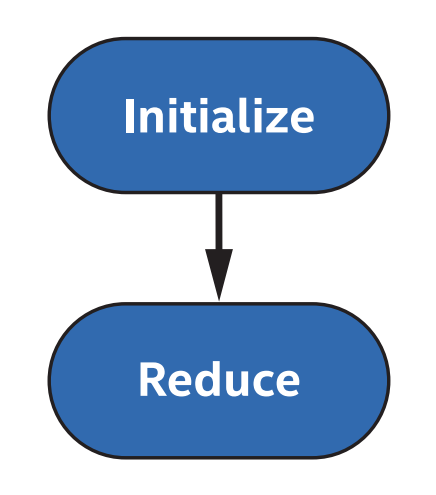
\includegraphics[width=0.2\textwidth]{content/chapter-8/images/2}
\end{center}

对于每个模式,我们将展示三种不同的实现。第一个实现将使用顺序队列,第二个将使用基于事件的依赖项,最后一个实现将使用缓冲区和访问器来表示命令组之间的数据依赖关系。\par

\hspace*{\fill} \par %插入空行
图8-2 “Y”模式依赖
\begin{center}
	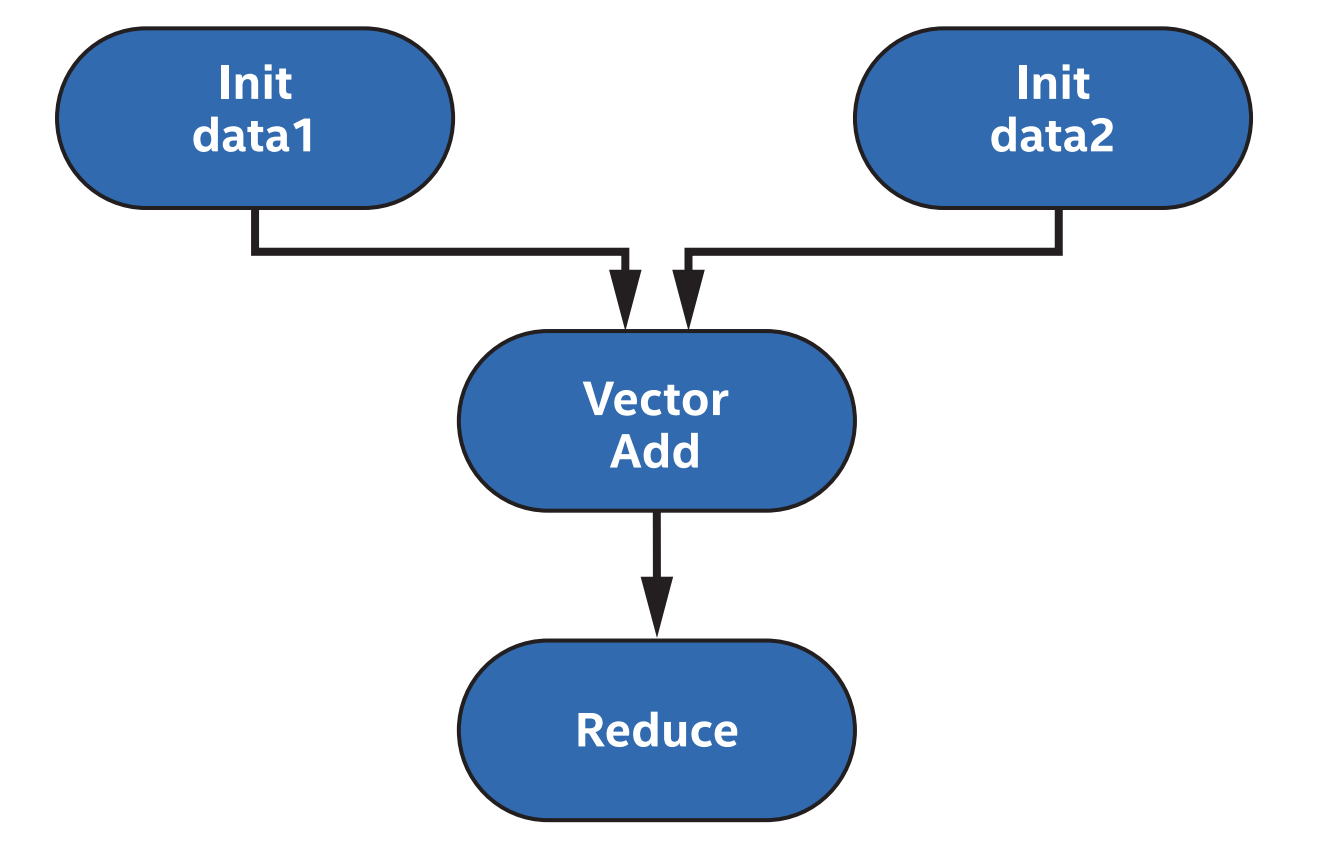
\includegraphics[width=0.5\textwidth]{content/chapter-8/images/3}
\end{center}

\hspace*{\fill} \par %插入空行
图8-3 具有有序队列的线性依赖链
\begin{lstlisting}[caption={}]
constexpr int N = 42;

queue Q{property::queue::in_order()};

int *data = malloc_shared<int>(N, Q);

Q.parallel_for(N, [=](id<1> i) { data[i] = 1; });

Q.single_task([=]() {
	for (int i = 1; i < N; i++)
		data[0] += data[i];
});

Q.wait();

assert(data[0] == N);
\end{lstlisting}

如图8-3所示,使用有序队列表示线性依赖链。这个示例非常简单,因为有序队列的语义可以保证命令组之间的连续执行顺序。我们提交的第一个内核将数组的元素初始化为1。下一个内核取这些元素,并将它们加起来成为第一个元素。由于队列是有序的,不需要做任何其他事情来表示第二个内核在第一个内核完成之前不应该执行。最后,等待队列完成它的所有任务,并检查是否获得了预期的结果。\par

\hspace*{\fill} \par %插入空行
图8-4 与事件线性相关的链
\begin{lstlisting}[caption={}]
constexpr int N = 42;

queue Q;

int *data = malloc_shared<int>(N, Q);

auto e = Q.parallel_for(N, [=](id<1> i) { data[i] = 1; });

Q.submit([&](handler &h) {
	h.depends_on(e);
	h.single_task([=]() {
		for (int i = 1; i < N; i++)
			data[0] += data[i];
	});
});

Q.wait();
assert(data[0] == N);
\end{lstlisting}

图8-4展示了使用无序队列和基于事件依赖的示例。这里,我们捕获第一次调用parallel\_for所返回的事件。然后,第二个内核能够指定对该事件的依赖,并通过将其作为参数传递给depends\_on来表示内核执行。我们将在图8-6中看到如何使用定义内核的一种快捷方法,来缩短第二个内核的表达式。\par

\hspace*{\fill} \par %插入空行
图8-5 带有缓冲区和访问器的线性依赖链
\begin{lstlisting}[caption={}]
constexpr int N = 42;
queue Q;

buffer<int> data{range{N}};

Q.submit([&](handler &h) {
	accessor a{data, h};
	h.parallel_for(N, [=](id<1> i) { a[i] = 1; });
});

Q.submit([&](handler &h) {
	accessor a{data, h};
	h.single_task([=]() {
		for (int i = 1; i < N; i++)
			a[0] += a[i];
	});
});

host_accessor h_a{data};
assert(h_a[0] == N);
\end{lstlisting}

图8-5使用缓冲区和访问器,重写了我们的线性依赖链示例。这里再次使用无序队列,但使用通过访问器指定的数据依赖项,而不是基于事件的依赖,对命令组的执行进行排序。第二个内核读取第一个内核产生的数据,运行时可以看到这一点,因为基于相同的底层缓冲区对象声明的访问器。这里与前面的示例不同,不需要等待队列完成所有任务。相反,这里使用主机访问器定义了数据之间的依赖关系,并在主机上计算出第二个内核的正确输出,并使用断言来判断内核给出的答案是否正确。请注意,虽然主机访问器提供了主机上数据的视图,但如果在创建缓冲区时指定了原始主机内存,就不能保证已经更新了原始主机内存。除非先销毁缓冲区,或者使用更高级的机制(如第7章中描述的互斥机制),否则无法安全地访问原始主机内存。\par

\hspace*{\fill} \par %插入空行
图8-6 有序队列的“Y”模式
\begin{lstlisting}[caption={}]
constexpr int N = 42;

queue Q{property::queue::in_order()};

int *data1 = malloc_shared<int>(N, Q);
int *data2 = malloc_shared<int>(N, Q);

Q.parallel_for(N, [=](id<1> i) { data1[i] = 1; });

Q.parallel_for(N, [=](id<1> i) { data2[i] = 2; });

Q.parallel_for(N, [=](id<1> i) { data1[i] += data2[i]; });

Q.single_task([=]() {
	for (int i = 1; i < N; i++)
		data1[0] += data1[i];
	data1[0] /= 3;
});

Q.wait();
assert(data1[0] == N);
\end{lstlisting}

如图8-6所示,使用有序队列表示“Y”模式。本例中,声明了两个数组data1和data2。然后定义两个内核,每个内核将初始化其中一个数组。这些内核并不相互依赖,但是由于队列是有序的,所以内核必须逐个地执行。而且,交换这两个内核的顺序是完全合法的。第二个内核执行之后,第三个内核将第二个数组的元素添加到第一个数组的元素中。最后一个内核函数将第一个数组的元素求和,从而得到与我们在线性相关链的例子中相同的结果。这个求和内核依赖于前面的内核,但是这个线性链也可以让有序队列捕获。最后,等待所有的内核都完成并验证我们是否成功地计算出了“魔数”。\par

\hspace*{\fill} \par %插入空行
图8-7 事件方式的“Y”模式
\begin{lstlisting}[caption={}]
constexpr int N = 42;
queue Q;

int *data1 = malloc_shared<int>(N, Q);
int *data2 = malloc_shared<int>(N, Q);

auto e1 = Q.parallel_for(N, 
			[=](id<1> i) { data1[i] = 1; });

auto e2 = Q.parallel_for(N, 
			[=](id<1> i) { data2[i] = 2; });

auto e3 = Q.parallel_for(range{N}, {e1, e2},
			[=](id<1> i) { data1[i] += data2[i]; });
	
Q.single_task(e3, [=]() {
	for (int i = 1; i < N; i++)
		data1[0] += data1[i];
	data1[0] /= 3;
});

Q.wait();
assert(data1[0] == N);
\end{lstlisting}

图8-7展示了另一种“Y”模式示例,使用了无序队列,而不是有序队列。由于队列的顺序,依赖关系不再是隐式的,因此必须使用事件显式地指定命令组之间的依赖关系。如图8-6所示,首先定义两个没有初始依赖关系的独立内核。用两个事件来表示这些内核,e1和e2。们定义第三个内核时,必须指定它依赖于前两个内核。这样做是因为它依赖于事件e1和e2在执行之前完成。但是,本例中使用一个快捷形式来指定这些依赖项,而不是处理程序的depends\_on方法。我们将事件作为额外参数传递给parallel\_for。想要一次传递多个事件,所以使用接受事件组的形式。幸运的是,现代C++通过表达式\{e1, e2\},会将其转换为适当的向量,简化了步操作。\par

\hspace*{\fill} \par %插入空行
图8-8 访问器的“Y”模式
\begin{lstlisting}[caption={}]
constexpr int N = 42;
queue Q;

buffer<int> data1{range{N}};
buffer<int> data2{range{N}};

Q.submit([&](handler &h) {
	accessor a{data1, h};
	h.parallel_for(N, [=](id<1> i) { a[i] = 1; });
});

Q.submit([&](handler &h) {
	accessor b{data2, h};
	h.parallel_for(N, [=](id<1> i) { b[i] = 2; });
});

Q.submit([&](handler &h) {
	accessor a{data1, h};
	accessor b{data2, h, read_only};
	h.parallel_for(N, [=](id<1> i) { a[i] += b[i]; });
});

Q.submit([&](handler &h) {
	accessor a{data1, h};
	h.single_task([=]() {
		for (int i = 1; i < N; i++)
			a[0] += a[i];
		a[0] /= 3;
	});
});

host_accessor h_a{data1};
assert(h_a[0] == N);
\end{lstlisting}

如图8-8所示,最后一个例子中,再次用缓冲区和访问器替换USM指针和事件。这个例子将两个数组data1和data2表示为缓冲区对象。内核不再使用快捷方法,因为必须将访问器与命令组处理程序关联起来。同样,第三个内核必须捕获对前两个内核的依赖关系。这里通过为缓冲区声明访问器来完成。因为之前已经为这些缓冲区声明了访问器,所以运行时能够正确地排列这些内核的执行顺序。此外,当声明访问器b时,还向运行时提供了额外的信息。添加了访问标记read\_only,让运行时知道只读取该数据,而不生成新值。正如在线性依赖链的缓冲区和访问器示例中所示,最终的内核通过更新第三个内核产生的值来对自身排序。通过声明一个主机访问器来获取计算的最终值,该访问器将等待最终内核完成执行,然后将数据移回主机,在那里可以读取数据,并断言内核是否计算出了正确的结果。\par 

\hspace*{\fill} \par %插入空行
\textbf{CG的各个部分是什么时候执行的?}

因为任务图是异步的,所以知道命令组究竟是什么时候执行是有意义的。目前为止,只要满足了内核的依赖关系,就可以执行内核,但是命令组的主机部分会发生什么呢?\par

当命令组提交到队列时,会立即在主机上执行(在submit返回之前)。命令组的主机部分只执行一次,在命令组中定义的任何内核或显式数据操作,都将排队在设备上执行。\par

































